\documentclass[aspectratio=169]{beamer}

\usetheme{Madrid}
\usecolortheme{seahorse}

\usepackage[utf8]{inputenc}
\usepackage[T1]{fontenc}
\usepackage{tikz}
\usetikzlibrary{arrows.meta, positioning, shapes.geometric}
\usepackage{listings}
\usepackage{xcolor}
\usepackage{graphicx}

\lstdefinestyle{yaml}{
  basicstyle=\ttfamily\tiny,
  keywordstyle=\color{blue},
  commentstyle=\color{gray},
  numbers=none,
  breaklines=true,
  frame=single,
  backgroundcolor=\color{black!4}
}

\title{Observability and Traffic Engineering}
\subtitle{Istio Service Mesh on Bookinfo}
\author{Diego, Esteban, Emmanuel}
\date{\today}

\begin{document}

\begin{frame}
  \titlepage
\end{frame}

\begin{frame}{Agenda}
  \tableofcontents
\end{frame}

% ============================================================
\section{Observability Stack}
% ============================================================

\begin{frame}{Mesh Architecture Under Observation}
  \centering
  \resizebox{!}{0.55\textheight}{%
  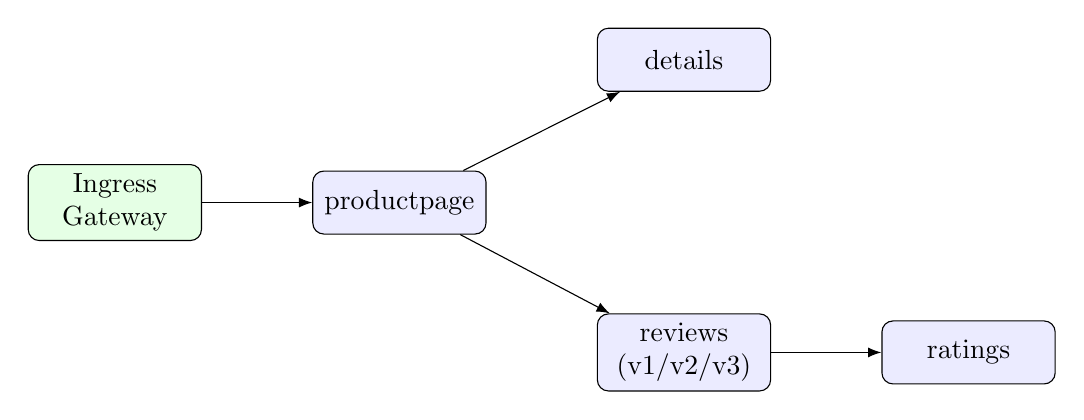
\begin{tikzpicture}[
      node distance=1.0cm and 1.4cm,
      svc/.style={draw, rounded corners, minimum width=2.2cm, minimum height=0.8cm, align=center, fill=blue!8},
      ext/.style={draw, rounded corners, minimum width=2.2cm, minimum height=0.8cm, align=center, fill=green!10}
    ]
    \node[ext] (gw) {Ingress\\Gateway};
    \node[svc, right=of gw] (pp) {productpage};
    \node[svc, above right=of pp] (det) {details};
    \node[svc, below right=of pp] (rev) {reviews\\(v1/v2/v3)};
    \node[svc, right=of rev] (rat) {ratings};

    \draw[-{Latex}] (gw) -- (pp);
    \draw[-{Latex}] (pp) -- (det);
    \draw[-{Latex}] (pp) -- (rev);
    \draw[-{Latex}] (rev) -- (rat);
  \end{tikzpicture}%
  }
  \vspace{0.3cm}
  \begin{center}
  \small Every hop is an Envoy sidecar call: Prometheus scrapes metrics, Jaeger\\
  collects spans, and Kiali renders the live graph from both.
  \end{center}
\end{frame}

\begin{frame}{Kiali: Service Topology}
  \begin{columns}
    \column{0.55\textwidth}
    \begin{itemize}
      \item Renders the live traffic graph from Prometheus data, refreshed every 15s.
      \item Shows per-edge request rate and success \%.
      \item Visualizes weighted routing (canary split) and header-based edges directly on the graph.
      \item \textbf{Istio Config} view lists every CRD (VirtualService, DestinationRule, Gateway, PeerAuthentication, Telemetry) with validation status.
    \end{itemize}
    \column{0.45\textwidth}
    \centering
    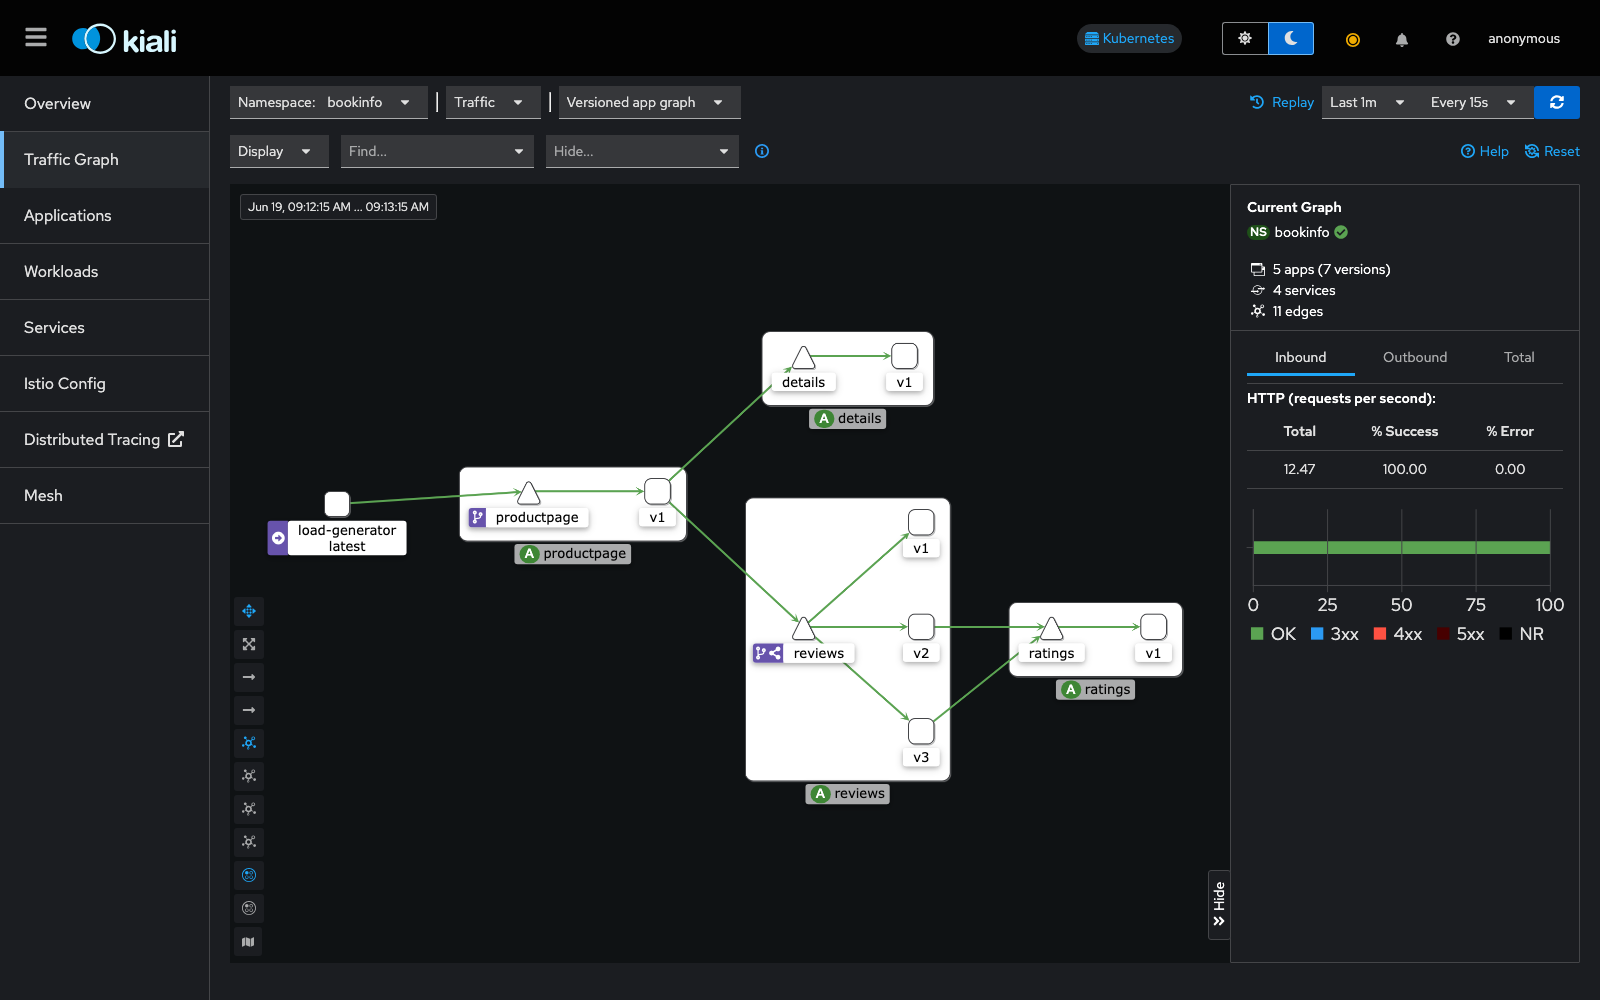
\includegraphics[width=\textwidth]{../docs/screenshots/routing/kiali_canary_topology.png}
  \end{columns}
\end{frame}

\begin{frame}{Grafana: Metrics Dashboards}
  \begin{columns}
    \column{0.55\textwidth}
    \begin{itemize}
      \item \texttt{06-install-metrics.sh} installs Prometheus and a custom \textbf{Bookinfo} dashboard.
      \item Three panels: request rate per service, 5xx error rate, and per-version \texttt{reviews} request rate.
      \item Standard Istio addon dashboards (Mesh, Service, Control Plane) also available.
      \item Used throughout the project to evidence canary splits and fault-injection scenarios.
    \end{itemize}
    \column{0.45\textwidth}
    \centering
    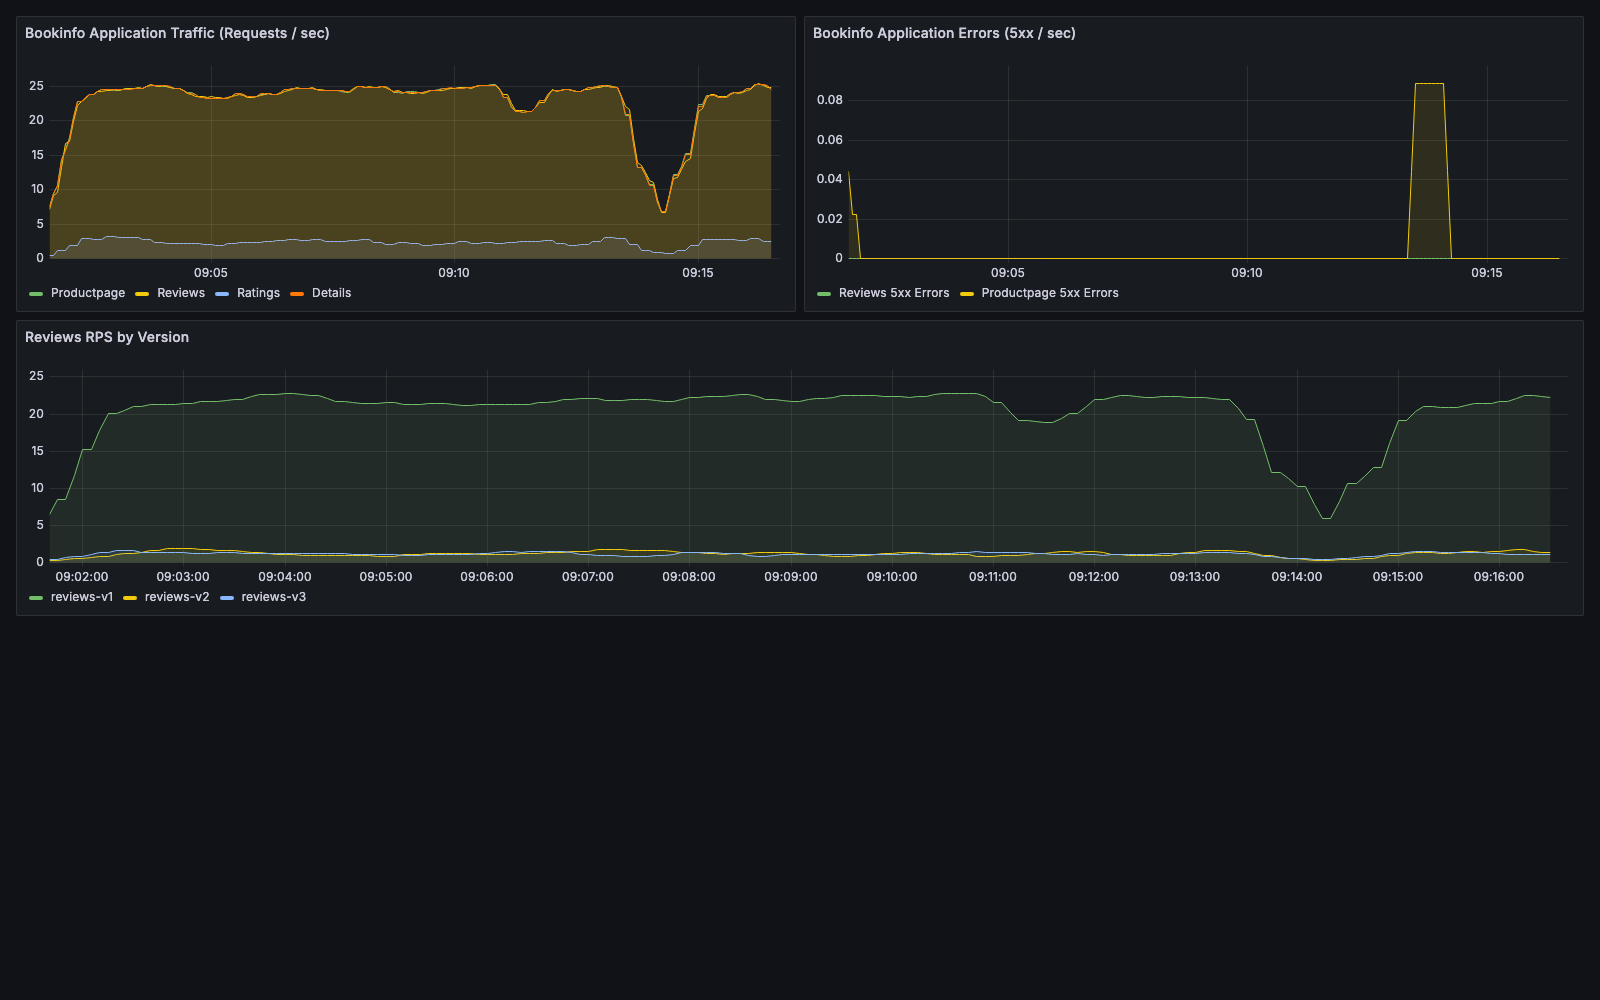
\includegraphics[width=\textwidth]{../docs/screenshots/routing/grafana_bookinfo_canary.png}
  \end{columns}
\end{frame}

\begin{frame}{Jaeger: Distributed Tracing}
  \begin{columns}
    \column{0.55\textwidth}
    \begin{itemize}
      \item \texttt{07-install-tracing.sh} installs single-binary Jaeger plus a \texttt{Telemetry} resource setting \textbf{100\% trace sampling} in \texttt{bookinfo} (vs. Istio's 1\% default).
      \item Services propagate W3C/B3 headers end-to-end, so one trace spans every hop.
      \item Search view: every request entering at \texttt{productpage}, fanning out to \texttt{details} and \texttt{reviews}.
    \end{itemize}
    \column{0.45\textwidth}
    \centering
    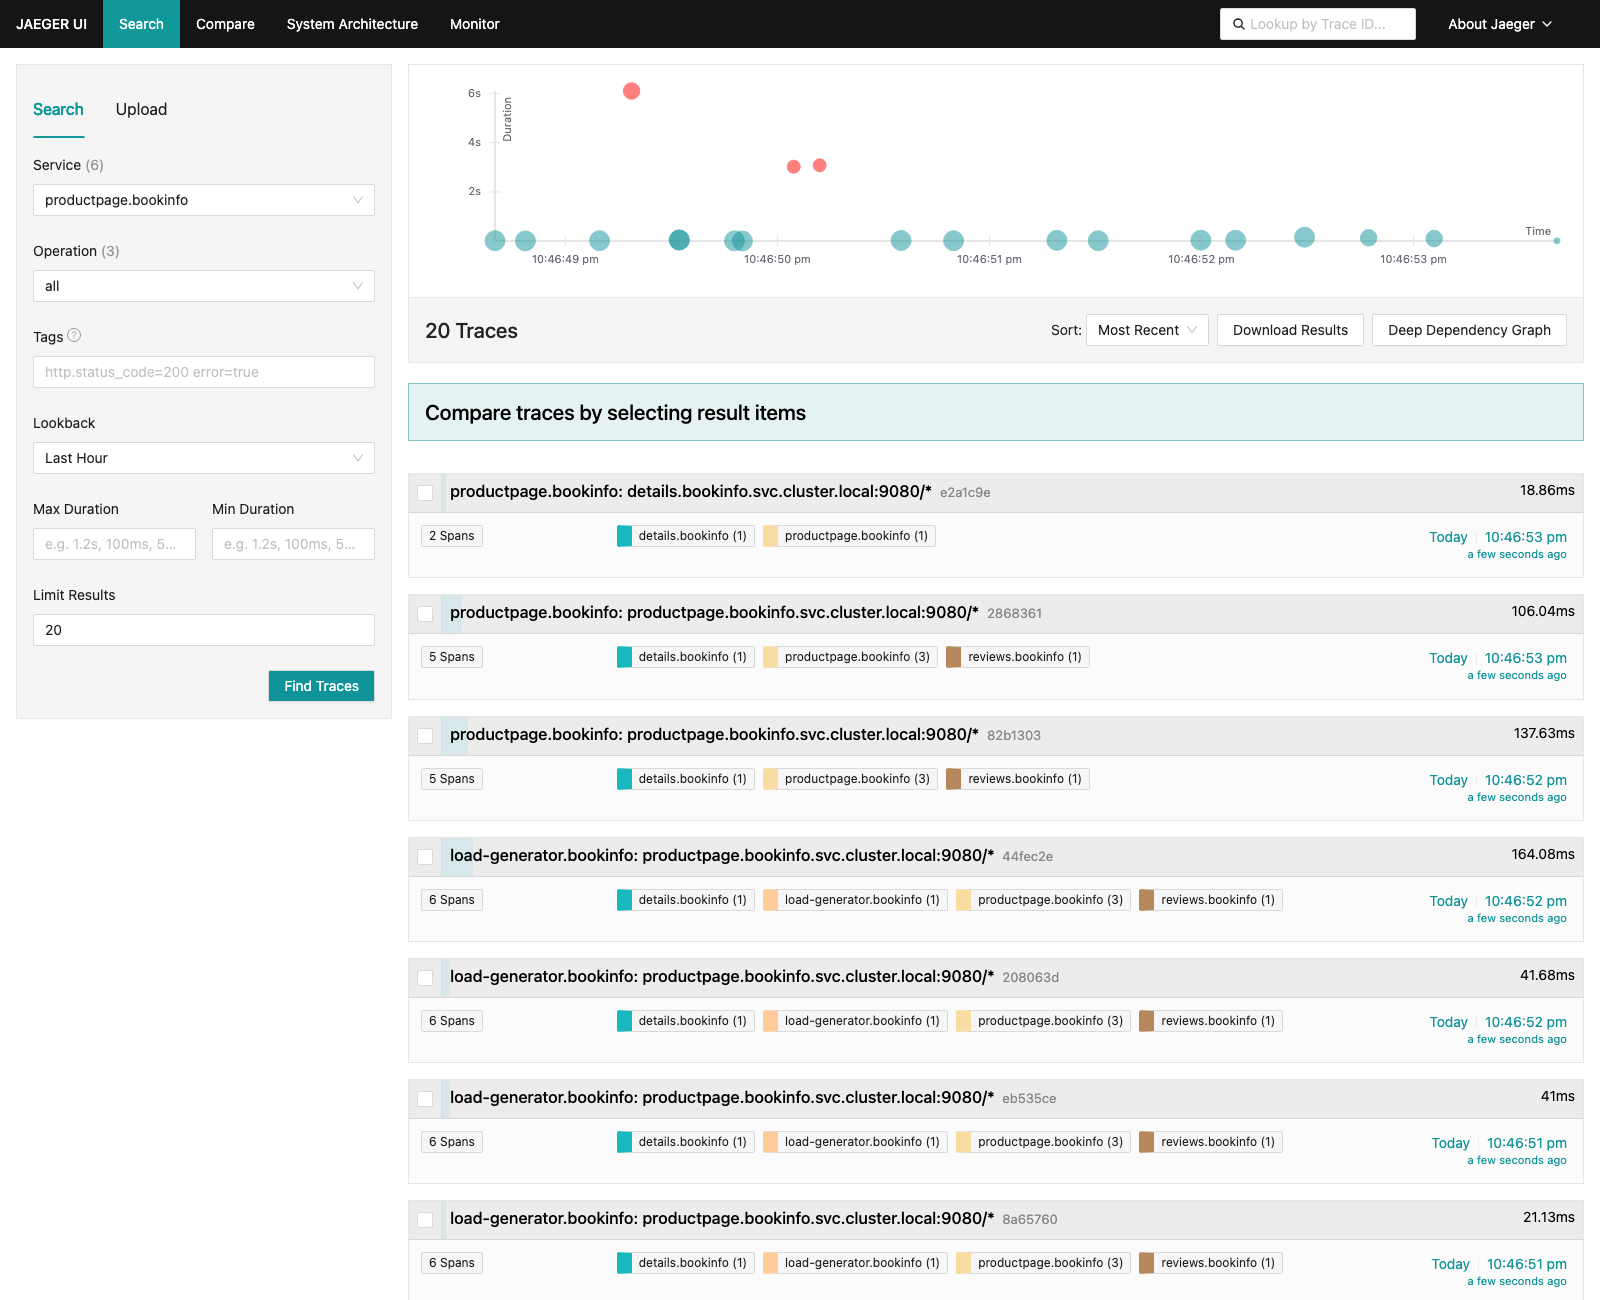
\includegraphics[width=\textwidth]{../docs/screenshots/tracing/jaeger_trace_list.png}
  \end{columns}
\end{frame}

\begin{frame}{Jaeger: Trace Waterfall}
  \begin{columns}
    \column{0.55\textwidth}
    \begin{itemize}
      \item Full call tree: \texttt{load-generator $\to$ productpage $\to$ \{details, reviews $\to$ ratings\}}.
      \item 5 services, 12 spans, per-span timing.
      \item Pinpoints exactly which downstream call is slow or failing --- e.g. a delayed \texttt{reviews $\to$ ratings} span surfaces immediately as an outlier.
    \end{itemize}
    \column{0.45\textwidth}
    \centering
    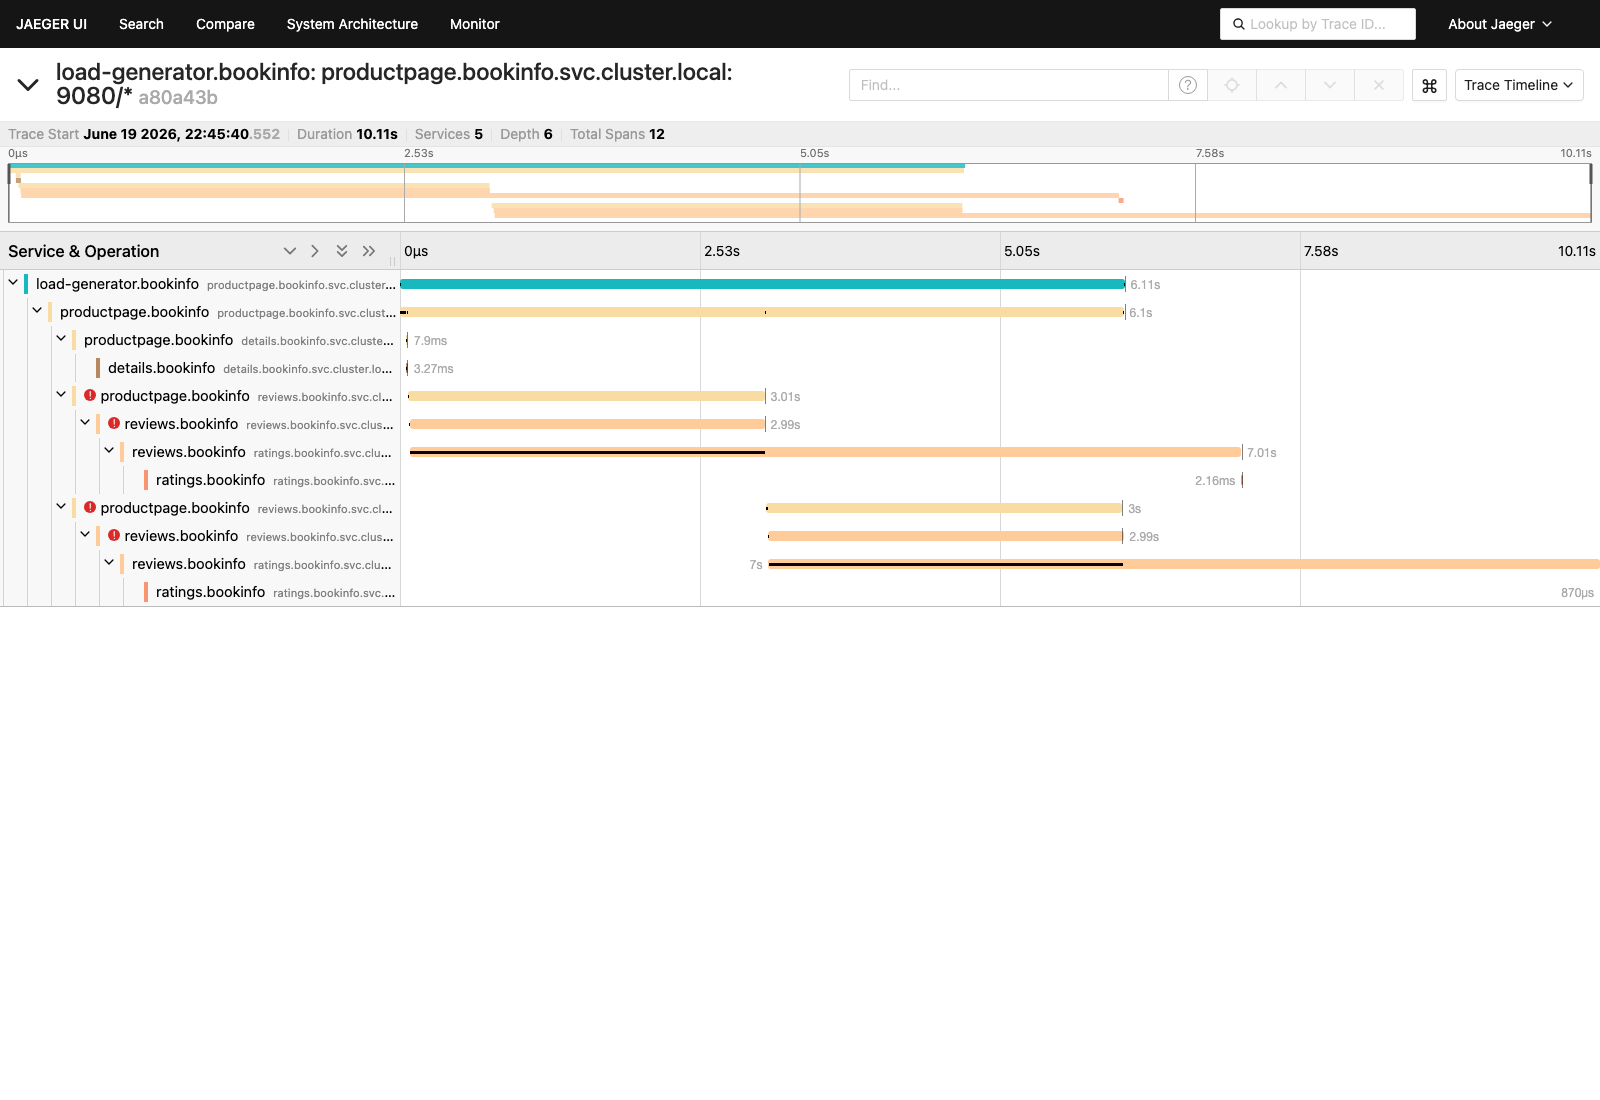
\includegraphics[width=\textwidth]{../docs/screenshots/tracing/jaeger_trace_detail.png}
  \end{columns}
\end{frame}

% ============================================================
\section{Traffic Engineering}
% ============================================================

\begin{frame}{Traffic Engineering: Overview}
  \begin{itemize}
    \item Goal: control how requests to \texttt{reviews} are split across \texttt{v1}/\texttt{v2}/\texttt{v3} without touching application code.
    \item Two complementary mechanisms, both expressed as Istio \texttt{VirtualService} resources:
    \begin{enumerate}
      \item \textbf{Canary release} --- weighted traffic split.
      \item \textbf{Header-based routing} --- deterministic routing for a specific user.
    \end{enumerate}
    \item Combined into a single \texttt{VirtualService} with priority-ordered HTTP match rules.
  \end{itemize}
\end{frame}

\begin{frame}[fragile]{Canary Release: 90/5/5 Split}
  \texttt{networking/virtual-service-canary.yaml}
  \begin{lstlisting}[style=yaml]
apiVersion: networking.istio.io/v1
kind: VirtualService
metadata:
  name: reviews-canary
spec:
  hosts: [reviews]
  http:
  - route:
    - destination: {host: reviews, subset: v1}
      weight: 90
    - destination: {host: reviews, subset: v2}
      weight: 5
    - destination: {host: reviews, subset: v3}
      weight: 5
  \end{lstlisting}
  \texttt{scripts/10-verify-canary.sh} samples 100 requests and asserts the
  v2+v3 ratio falls within $10\% \pm 5\%$.
\end{frame}

\begin{frame}[fragile]{Header-Based Routing}
  \texttt{networking/combined-virtual-service.yaml} --- priority order:
  \begin{enumerate}
    \item Header \texttt{end-user: jason} $\to$ 100\% to \texttt{reviews-v2}.
    \item Everything else $\to$ falls through to the 90/5/5 canary split.
  \end{enumerate}
  \begin{lstlisting}[style=yaml]
http:
  - name: header-based-routing
    match:
    - headers: {end-user: {exact: "jason"}}
    route:
    - destination: {host: reviews, subset: v2}
      weight: 100
  - name: canary-default-routing
    route:
    - destination: {host: reviews, subset: v1}
      weight: 90
    - destination: {host: reviews, subset: v2}
      weight: 5
    - destination: {host: reviews, subset: v3}
      weight: 5
  \end{lstlisting}
\end{frame}

\begin{frame}{Routing Decision Path}
  \centering
  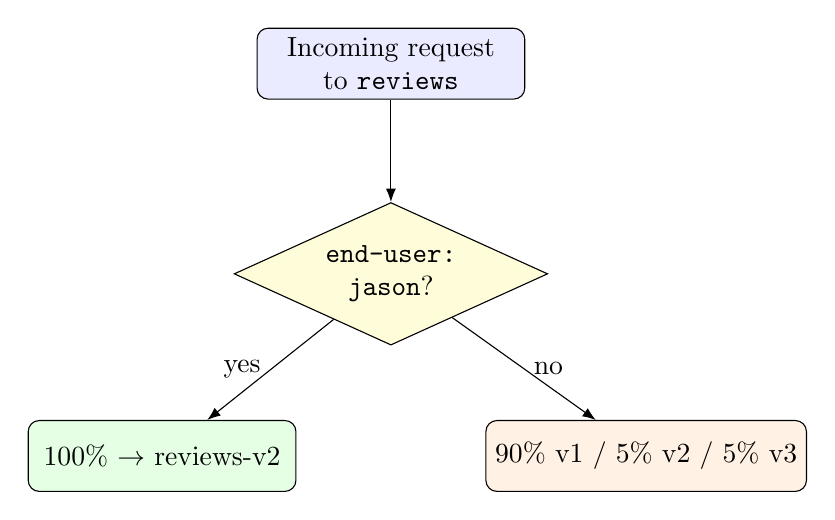
\begin{tikzpicture}[
      node distance=1.3cm and 2.0cm,
      box/.style={draw, rounded corners, minimum width=3.4cm, minimum height=0.9cm, align=center},
      dec/.style={draw, diamond, aspect=2.2, minimum width=3.6cm, align=center, fill=yellow!15}
    ]
    \node[box, fill=blue!8] (req) {Incoming request\\to \texttt{reviews}};
    \node[dec, below=of req] (chk) {\texttt{end-user:}\\\texttt{jason}?};
    \node[box, fill=green!10, below left=1.4cm and 0.2cm of chk] (v2) {100\% $\to$ reviews-v2};
    \node[box, fill=orange!10, below right=1.4cm and 0.2cm of chk] (canary) {90\% v1 / 5\% v2 / 5\% v3};

    \draw[-{Latex}] (req) -- (chk);
    \draw[-{Latex}] (chk) -- node[left]{yes} (v2);
    \draw[-{Latex}] (chk) -- node[right]{no} (canary);
  \end{tikzpicture}
  \vspace{0.3cm}
  \texttt{scripts/11-test-header-routing.sh} confirms both paths: an anonymous
  request gets any valid version, a \texttt{jason} request always gets \texttt{v2}.
\end{frame}

\begin{frame}{Observed Effect: Kiali Traffic Split}
  \centering
  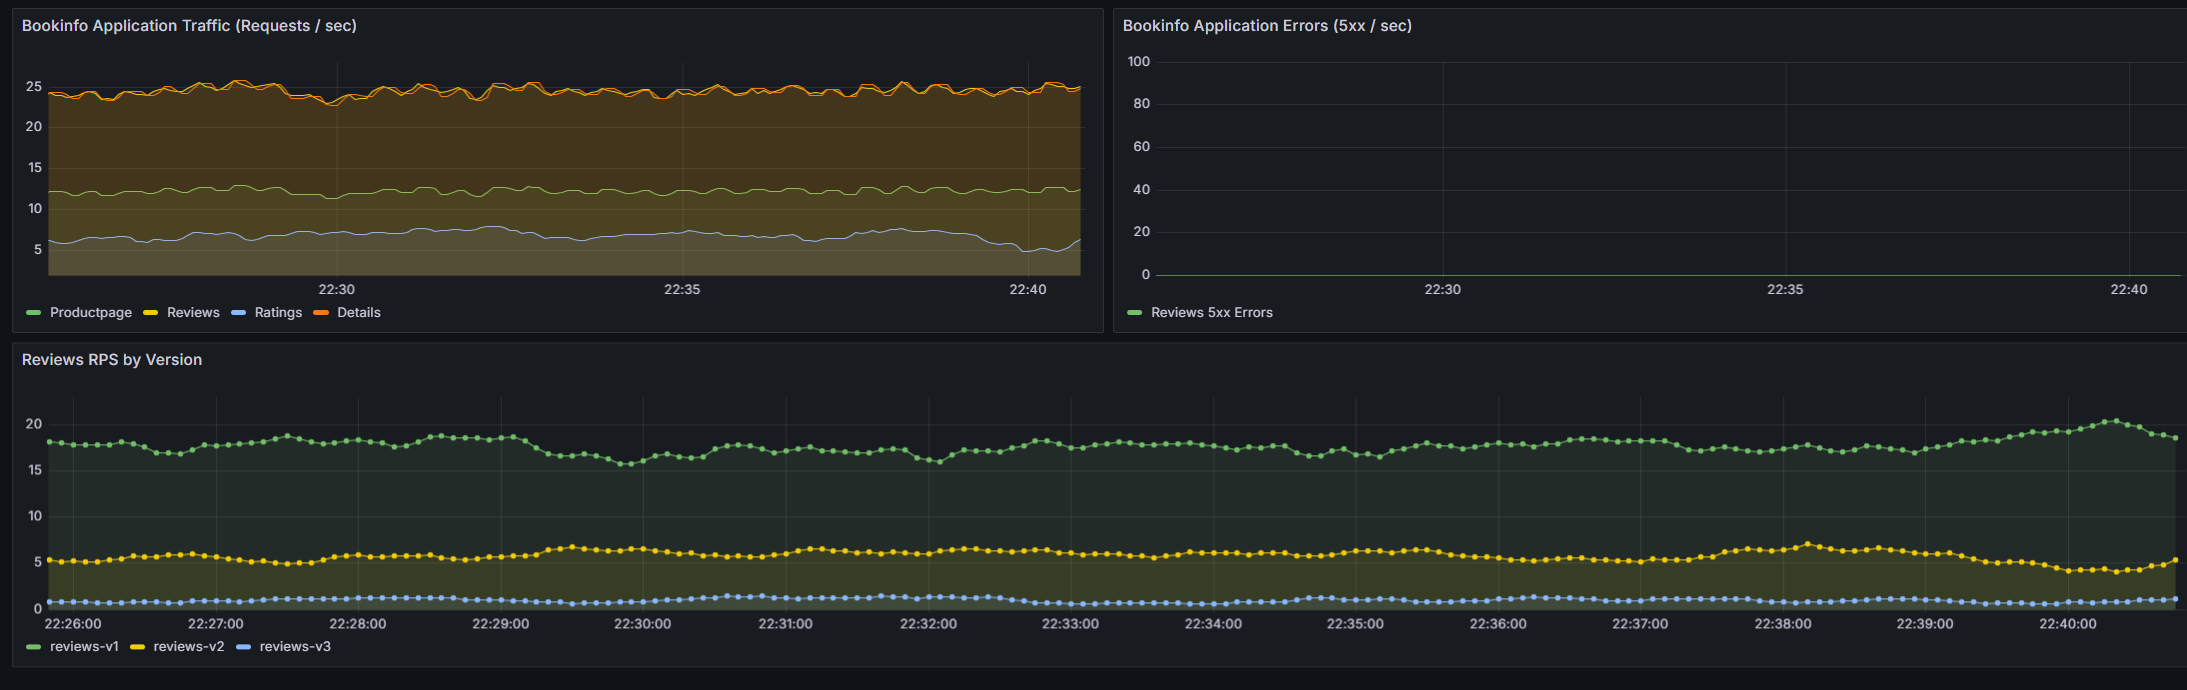
\includegraphics[width=0.7\textwidth]{../docs/screenshots/routing/kiali_traffic_split.png}
  \begin{center}
  \small Kiali renders both the weighted edges to v1/v2/v3 and the
  header-matched edge to v2 under load.
  \end{center}
\end{frame}

% ============================================================
\section{Live Demonstration}
% ============================================================

\begin{frame}{Live Demonstration}
  \begin{enumerate}
    \item Cluster, Istio, Bookinfo, metrics, and tracing already running
          (\texttt{scripts/run-all.sh}, lines 1--37).
    \item Apply the \textbf{canary} \texttt{VirtualService} and run
          \texttt{10-verify-canary.sh}.
    \item Apply the \textbf{combined header-based} \texttt{VirtualService} and run
          \texttt{11-test-header-routing.sh}.
    \item Observe the effect live in \textbf{Kiali}, \textbf{Grafana}, and \textbf{Jaeger}.
  \end{enumerate}
  \vspace{0.5cm}
  \centering
  \textit{No further slides --- switching to the terminal and browser.}
\end{frame}

\begin{frame}{Thank You}
  \centering
  \Large Questions?
\end{frame}

\end{document}
